\documentclass[a4paper]{report}

\usepackage[T1]{fontenc}
%\usepackage[bitstream-charter]{mathdesign}
\usepackage[english]{babel}
\usepackage[utf8]{inputenc}
\usepackage{a4wide}
%\usepackage{csquotes}
\usepackage [autostyle, english = american]{csquotes}
\MakeOuterQuote{"}
\usepackage[maxbibnames=99,style=authoryear]{biblatex}
\usepackage[pdfusetitle]{hyperref}
\usepackage{enumitem}
\usepackage[toc,page,title]{appendix}
\addbibresource{bib.bib}
\usepackage{caption}
\usepackage{subcaption}
\usepackage{gensymb}
\usepackage{varwidth}
\usepackage{tabularx}
\usepackage{float}
\usepackage{tikz}
\usepackage{minted}
\usetikzlibrary{er,positioning}
\definecolor{mypurple}{RGB}{117,112,179}
\input{version}

\newcommand{\onpage}[1]{\ref{#1} on page~\pageref{#1}}

\newcommand{\DP}{Douglas \& Peucker}
\newcommand{\VW}{Visvalingam--Whyatt}
\newcommand{\WM}{Wang--M{\"u}ller}

\newcommand{\MYTITLE}{Cartographic Generalization of Lines using free software (example of rivers)}
\newcommand{\MYAUTHOR}{Motiejus Jakštys}

\title{\MYTITLE}
\author{\MYAUTHOR}
\date{\VCDescribe}

\begin{document}

\begin{titlepage}
    \begin{center}
        
\includegraphics[width=0.4\textwidth]{vu}

        \huge
        \textbf{\MYTITLE} \\[4ex]

        \LARGE
        \textbf{\MYAUTHOR} \\[8ex]

        \vfill

        A thesis presented for the degree of\\
        Master in Cartography \\[3ex]

        \large
        \VCDescribe
    \end{center}
\end{titlepage}

\begin{abstract}
\label{sec:abstract}
Current open-source line generalization solutions have their roots in
    mathematics and geometry, and are not fit for natural objects like rivers
    and coastlines. This paper discusses our implementation of {\WM} algorithm
    under and open-source license, explains things that we would had
    appreciated in the original paper and compares our results to different
    generalization algorithms.
\end{abstract}

\newpage

\tableofcontents
\listoffigures

\newpage

\chapter{Introduction}
\label{sec:introduction}

When creating small-scale maps, often the detail of the data source is greater
than desired for the map. This becomes especially acute for natural features
that have many bends, like coastlines, rivers and forest boundaries.

To create a small-scale map from a large-scale data source, these features need
to be generalized: detail should be reduced. However, while doing so, it is
important to preserve the "defining" shape of the original feature, otherwise
the result will look unrealistic.

For example, if a river is nearly straight, it should be nearly straight after
generalization, otherwise a too straightened river will look like a canal.
Conversely, if the river is highly wiggly, the number of bends should be
reduced, but not removed.

Generalization problem for other objects can often be solved by other
non-geometric means:

\begin{itemize}
    \item Towns and cities can be filtered and generalized by number of
        inhabitants.
    \item Roads can be eliminated by the road length, number of lanes, or
        classification of the road (local, regional, international).
\end{itemize}

Natural line generalization problem can be viewed as having two competing
goals:

\begin{itemize}
    \item Reduce detail by removing or simplifying "less important" features.
    \item Retain enough detail, so the original is still recognize-able.
\end{itemize}

Given the discussed complexities, a fine line between under-generalization
(leaving object as-is) and over-generalization (making a straight line) must be
found. Therein lies the complexity of generalization algorithms: all have
different trade-offs.

\chapter{Literature review}
\label{sec:literature-review}

A number of cartographic line generalization algorithms have been researched.
The "classical" ones are {\DP} and {\VW}.

\section{{\DP} and {\VW}}

\cite{douglas1973algorithms} and \cite{visvalingam1993line} are "classical"
line generalization computer graphics algorithms. They are relatively simple to
implement, require few runtime resources. Both of them accept only a single
parameter, based on desired scale of the map, which makes them very simple to
adjust for different scales.

Both algorithms are part of PostGIS, a free-software GIS suite:
\begin{itemize}
    \item \cite{douglas1973algorithms} via
        \href{https://postgis.net/docs/ST_Simplify.html}{PostGIS Simplify}.

    \item \cite{visvalingam1993line} via
        \href{https://postgis.net/docs/ST_SimplifyVW.html}{PostGIS SimplifyVW}.
\end{itemize}

Since both algorithms produce jagged output lines, it is worthwhile to process
those through a widely available \cite{chaikin1974algorithm} smoothing
algorithm via \href{https://postgis.net/docs/ST_ChaikinSmoothing.html}{PostGIS
ChaikinSmoothing}.

Even though {\DP} and {\VW} are simple to understand and computationally
efficient, they have serious deficiencies for cartographic natural line
generalization.

<TODO: expand on deficiencies>

\section{Modern approaches}

Due to their simplicity and ubiquity, {\DP} and {\VW} have been established as
go-to algorithms for line generalization. During recent years, alternatives
have emerged. These modern replacements fall into roughly two categories:

\begin{itemize}
    \item Cartographic knowledge was encoded to an algorithm (bottom-up
        approach). One among these are \cite{wang1998line}.
    \item Mathematical shape transformation which yields a more cartographic
        result. E.g. \cite{jiang2003line}, \cite{dyken2009simultaneous},
        \cite{mustafa2006dynamic}, \cite{nollenburg2008morphing}.
\end{itemize}

Authors of most of the aforementioned articles have implemented the
generalization algorithm, at least to generate the visuals in the articles.
However, I wasn't able to find code for any of those to evaluate with my
desired data set, or use as a basis for my own maps. \cite{wang1998line} is
available in a commercial product.

Lack of robust openly available generalization algorithm implementations poses
a problem for map creation with free software: there is not a similar
high-quality simplification algorithm to create down-scaled maps, so any
cartographic work, which uses line generalization as part of its processing,
will be of sub-par quality. We believe that availability of high-quality
open-source tools is an important foundation for future cartographic
experimentation and development, thus it it benefits the cartographic society
as a whole.

\chapter{Methodology}
\label{sec:methodology}

The original \cite{wang1998line} leaves something to be desired for a practical
implementation: it is not straightforward to implement the algorithm from the
paper alone.

Explanations in this document are meant to expand, rather than substitute, the
original description in \cite{wang1998line}. Therefore familiarity with the
original paper is assumed, and, for some sections, having it close-by is
necessary to meaningfully follow this document.

In this paper we describe {\WM} in a detail that is more useful for algorithm:
each section will be expanded, with more elaborate and exact illustrations for
every step of the algorithm.

Algorithms discussed in this paper assume Euclidean geometry.

\section{Vocabulary and terminology}

This section defines vocabulary and terms as defined in the rest of the paper.

\begin{description}

    \item[Vertex] is a point on a plane, can be expressed by a pair of $(x,y)$
        coordinates.

    \item[Line Segment (or Segment)] joins two vertices by a straight line. A
        segment can be expressed by two coordinate pairs: $(x_1, y_1)$ and
        $(x_2, y_2)$. Line Segment and Segment are used interchangeably.

    \item[Line] represents a single linear feature in the real world. For
        example, a river or a coastline. {\tt LINESTRING} in GIS terms.

        Geometrically, A line is a series of connected line segments, or,
        equivalently, a series of connected vertices. Each vertex connects to
        two other vertices, except those vertices at either ends of the line:
        these two connect to a single other vertex.

    \item[Bend] is a subset of a line that humans perceive as a curve. For the
        purpose of this paper, the geometric definition is complex and is
        discussed in section~\onpage{sec:definition-of-a-bend}.

\end{description}

\section{Automated tests}
\label{sec:automated-tests}

As part of the algorithm realization, an automated test suite has been
developed. Shapes to test each function have been hand-crafted and expected
results have been manually calculated. The test suite executes parts of the
algorithm against a predefined set of geometries, and asserts that the output
matches the resulting hand-calculated geometry.

The full set of test geometries is visualized in
figure~\onpage{fig:test-figures}. The figure includes arrows depicting line
direction.

\begin{figure}[h]
    \centering
    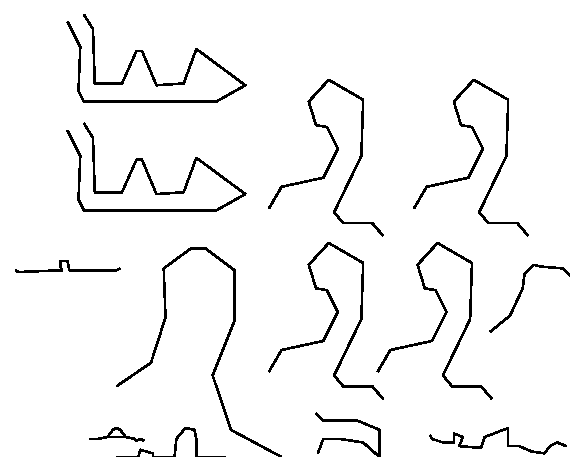
\includegraphics[width=\linewidth]{test-figures}
    \caption{Line geometries for automated test cases}
    \label{fig:test-figures}
\end{figure}

The full test suite can be executed with a single command, and completes in a
few seconds. Having an easily accessible test suite boosts confidence that no
unexpected bugs have snug in while modifying the algorithm.

\chapter{Description of the implementation}

Like alluded in section~\onpage{sec:introduction}, \cite{wang1998line} paper
skims over certain details, which are important to implement the algorithm.
This section goes through each algorithm stage, illustrating the intermediate
steps and explaining the author's desiderata for a more detailed description.

Illustrations of the following sections are extracted from the automated test
cases, which were written during the algorithm implementation (as discussed in
section~\onpage{sec:automated-tests}).

Lines in illustrations are black, and bends are heavily colored after
converting them to polygons. Bends are converted to polygons (for illustration
purposes) using the following algorithm:

\begin{itemize}
    \item Join the first and last vertices of the bend, creating a polygon.
    \item Color the polygons using distinct colors.
\end{itemize}

\section{Definition of a Bend}
\label{sec:definition-of-a-bend}

The original article describes:

\begin{displayquote}[\cite{wang1998line}][]
    A bend can be defined as that part of a line which contains a number of
    subsequent vertices, with the inflection angles on all vertices included in
    the bend being either positive or negative and the inflection of the bend's
    two end vertices being in opposite signs.
\end{displayquote}

While it gives a good intuitive understanding of what the bend is, some more
technical details would be appreciated.

Figure~\ref{fig:fig8-definition-of-a-bend} illustrates article's figure 8,
but with bends colored as polygons: each color is a distinctive bend.

\begin{figure}[h]
    \centering
    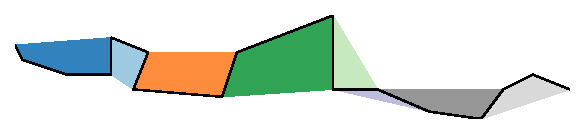
\includegraphics[width=\linewidth]{fig8-definition-of-a-bend}
    \caption{Originally figure 8: detected bends are highlighted}
    \label{fig:fig8-definition-of-a-bend}
\end{figure}

Once the intuitive definition is established, here are some non-obvious
characteristics that are necessary when writing code to detect the bends:

\begin{itemize}

    \item End segments of each line should also belong to bends. That way, all
        segments belong to 1 or 2 bends.

    \item First and last segments of each bend (except for the two end-line
        segments) is also the first vertex of the next bend.
\end{itemize}

Properties above may be apparent when looking at illustrations at this article
or reading here, but they are nowhere as such when looking at the original
article.

\section{Gentle Inflection at End of a Bend}

The gist of the section is in the original article:

\begin{displayquote}[\cite{wang1998line}][]
    But if the inflection that marks the end of a bend is quite small, people
    would not recognize this as the bend point of a bend
\end{displayquote}

Figure~\ref{fig:fig5-gentle-inflection} visualizes original paper's Figure 5,
when a single vertex is moved outwards the end of the bend.

\begin{figure}[h]
    \centering
    \begin{subfigure}[b]{.49\textwidth}
        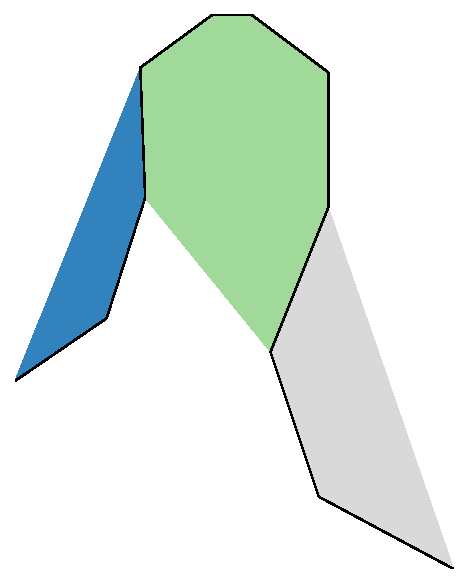
\includegraphics[width=\textwidth]{fig5-gentle-inflection-before}
        \caption{Before applying the inflection rule}
    \end{subfigure}
    \hfill
    \begin{subfigure}[b]{.49\textwidth}
        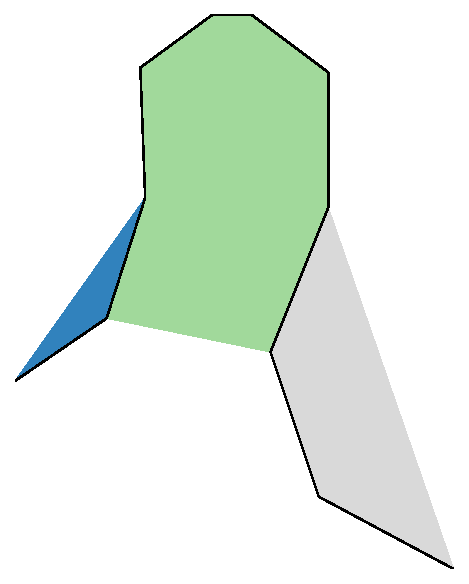
\includegraphics[width=\textwidth]{fig5-gentle-inflection-after}
        \caption{After applying the inflection rule}
    \end{subfigure}
    \caption{Originally figure 5: gentle inflections at the ends of the bend}
    \label{fig:fig5-gentle-inflection}
\end{figure}

The illustration for this section was clear, but insufficient: it does not
specify how many vertices should be included when calculating the end-of-bend
inflection. We chose the iterative approach --- as long as the angle is "right"
and the distance is decreasing, the algorithm should keep re-assigning vertices
to different bends; practically not having an upper bound on the number of
iterations.

To prove that the algorithm implementation is correct for multiple vertices,
additional example was created, and illustrated in
figure~\ref{fig:inflection-1-gentle-inflection}: the rule re-assigns two
vertices to the next bend instead of one.

\begin{figure}[h]
    \centering
    \begin{subfigure}[b]{.45\textwidth}
        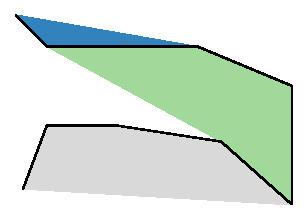
\includegraphics[width=\textwidth]{inflection-1-gentle-inflection-before}
        \caption{Before applying the inflection rule}
    \end{subfigure}
    \hfill
    \begin{subfigure}[b]{.45\textwidth}
        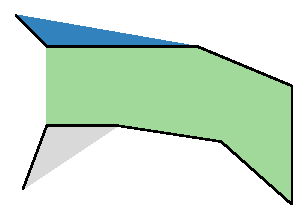
\includegraphics[width=\textwidth]{inflection-1-gentle-inflection-after}
        \caption{After applying the inflection rule}
    \end{subfigure}
    \caption{Gentle inflection at the end of the bend when multiple vertices is moved.}
    \label{fig:inflection-1-gentle-inflection}
\end{figure}


\section{Self-line Crossing When Cutting a Bend}

\section{Attributes of a Single Bend}

\section{Shape of a Bend}

\section{The Context of a Bend: Isolated and Similar Bends}

\section{Elimination Operator}

\section{Combination Operator}

\section{Exaggeration Operator}

\chapter{Program Implementation}

\chapter{Results of Experiments}

\chapter{Conclusions}
\label{sec:conclusions}

\chapter{Related Work and future suggestions}
\label{sec:related_work}

\printbibliography

\begin{appendices}

\chapter{Code listings}

We strongly believe in the ability to reproduce the results is critical for any
    scientific work. To make it possible for this paper, all source files and
    accompanying scripts have been attached to the PDF. To re-generate this
    document and its accompanying graphics, run this script (assuming name of
    this document is {\tt mj-msc-full.pdf}):

\inputminted[fontsize=\small]{bash}{extract-and-generate}

This was tested on Linux Debian 11 with upstream packages only.

\end{appendices}
\end{document}
